% !TEX root = MAIN.tex

\chapter{Software Overview}
\label{chapter:overview}

\section{Function and Purpose}

The FAQAS activity concerns the investigation of mutation testing as a method to evaluate the quality of software test suites and mutation testing as a method to derive new software test cases.

The \FAQAS shall support a code-driven and data-driven mutation testing methodology that integrates and extends state-of-art solutions. The reference methodology has been described in D2. The methodology enables a scalable and accurate mutation testing process even when the software under test is large and characterized by test suites requiring long execution time.

The end-user of the \FAQAS is a software engineer (i.e., a professional with a master degree in informatics or related fields)  who aims to evaluate the quality of the test suite developed for a flight software component or system. Hereafter, the end-user of \FAQAS is referred to as \emph{the engineer}.

Since \FAQAS implements two distinct features, code-driven mutation testing and data-driven mutation testing, this document contains two separate sections, each one concerning one of the two features: Section~\ref{sec:codeDriven} concerns code-driven mutation testing, Section~\ref{sec:dataDriven} concerns data-driven mutation testing.

The requirements defined in this chapter are univocally identified by the paragraph id appearing on the left.

\section{General Capabilities}

\RQ{} \FAQAS shall support test suite evaluation based on code mutation.

\RQ{} \FAQAS shall support test suite augmentation based on code mutation.

\RQ{} \FAQAS shall support test suite evaluation based on data mutation.

\RQ{} \FAQAS should support test suite augmentation based on data mutation.

\REVISION{P-8 P-13}{\RQ{} \FAQAS shall implement the code-driven test suite evaluation and test suite augmentation steps depicted in Figure~\ref{fig:code:process_eva} and Figure~\ref{fig:code:process_aug}. Detailed explanation is provided in D2 Chapter 1.}

\begin{figure}
	\centering
		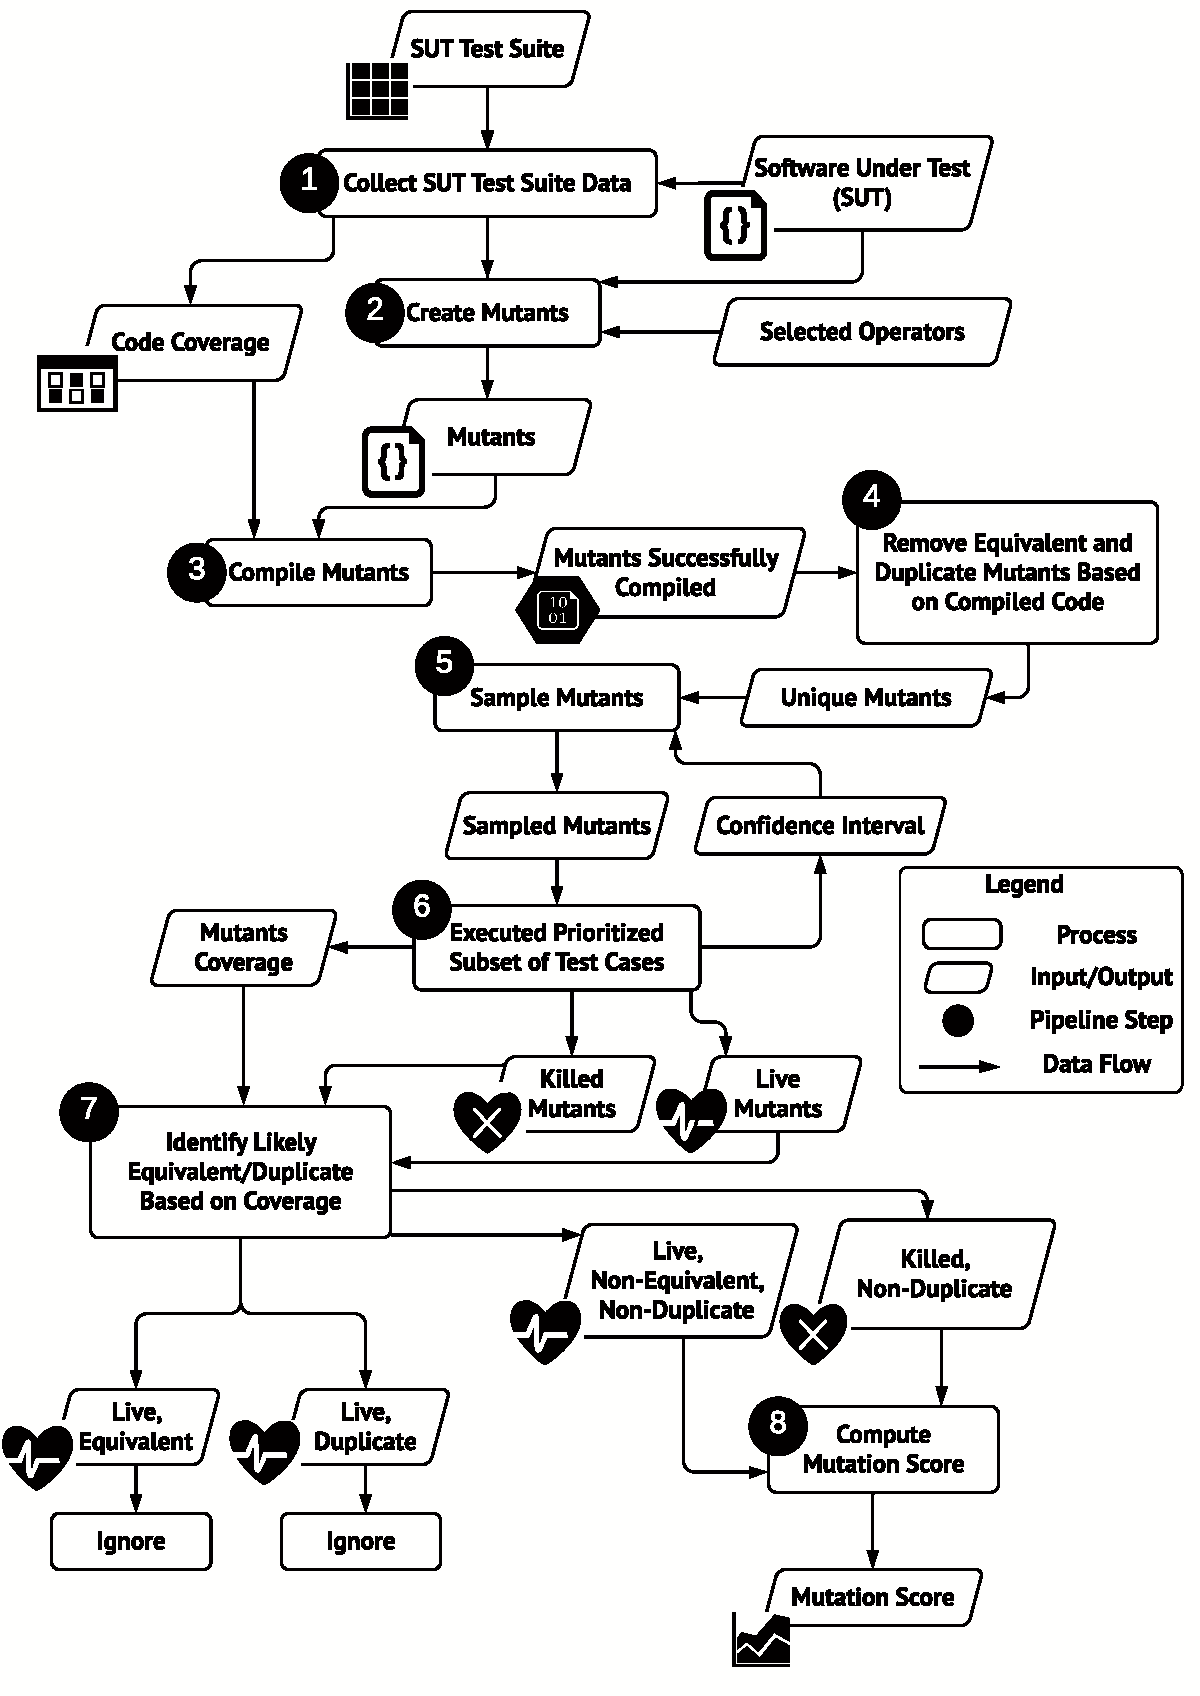
\includegraphics[width=12cm]{images/MASS_Approach}
		\caption{Code-driven Mutation Testing Process: Evaluation}
		\label{fig:code:process_eva}
	\end{figure}

\begin{figure}
	\centering
		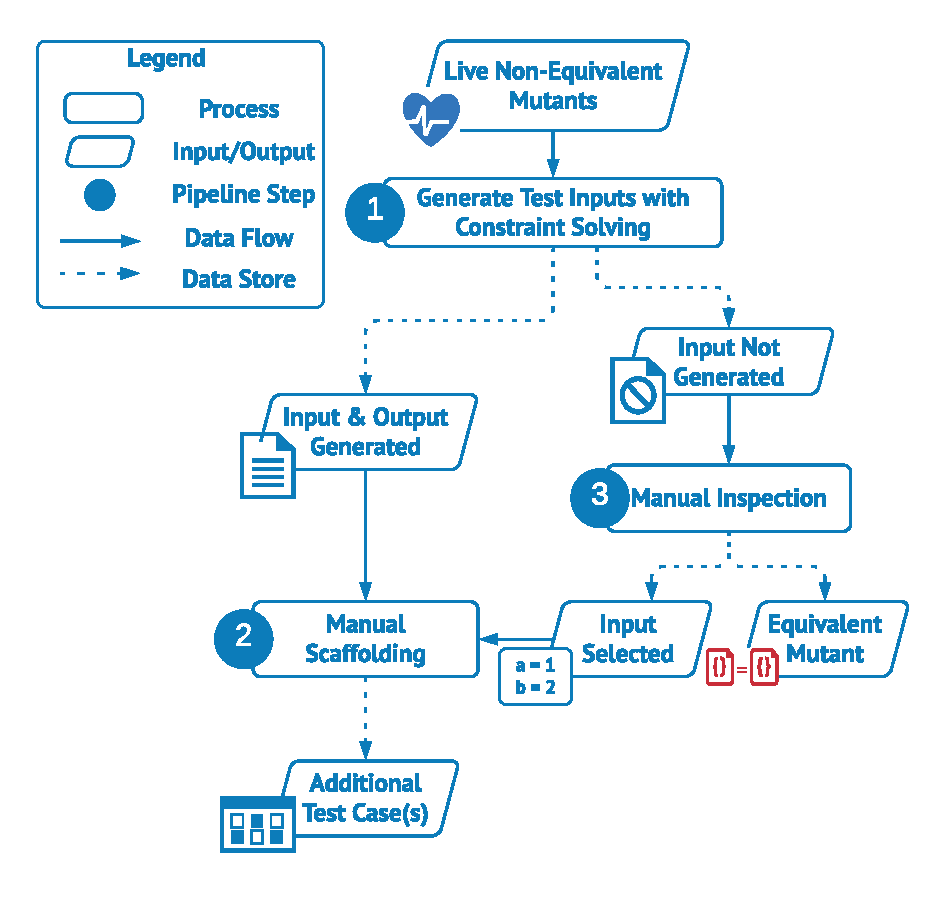
\includegraphics[width=12cm]{images/MT2}
		\caption{Code-driven Mutation Testing Process: Augmentation}
		\label{fig:code:process_aug}
	\end{figure}


\REVISION{P-8}{\RQ{} \FAQAS shall implement the data-driven test suite evaluation and test suite augmentation steps depicted in Figure~\ref{fig:data:process_eva} and Figure~\ref{fig:data:process_aug}. Detailed explanation is provided in D2 Chapter 2.}

\begin{figure}
	\centering
		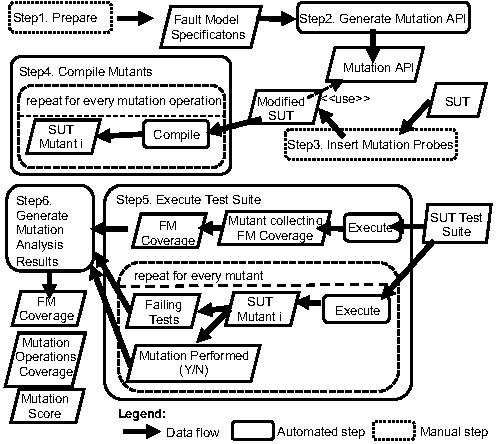
\includegraphics[width=12cm]{images/dataDrivenBufferProcess}
		\caption{Data-driven Mutation Testing Process: Evaluation}
		\label{fig:data:process_eva}
	\end{figure}

	\begin{figure}
		\centering
			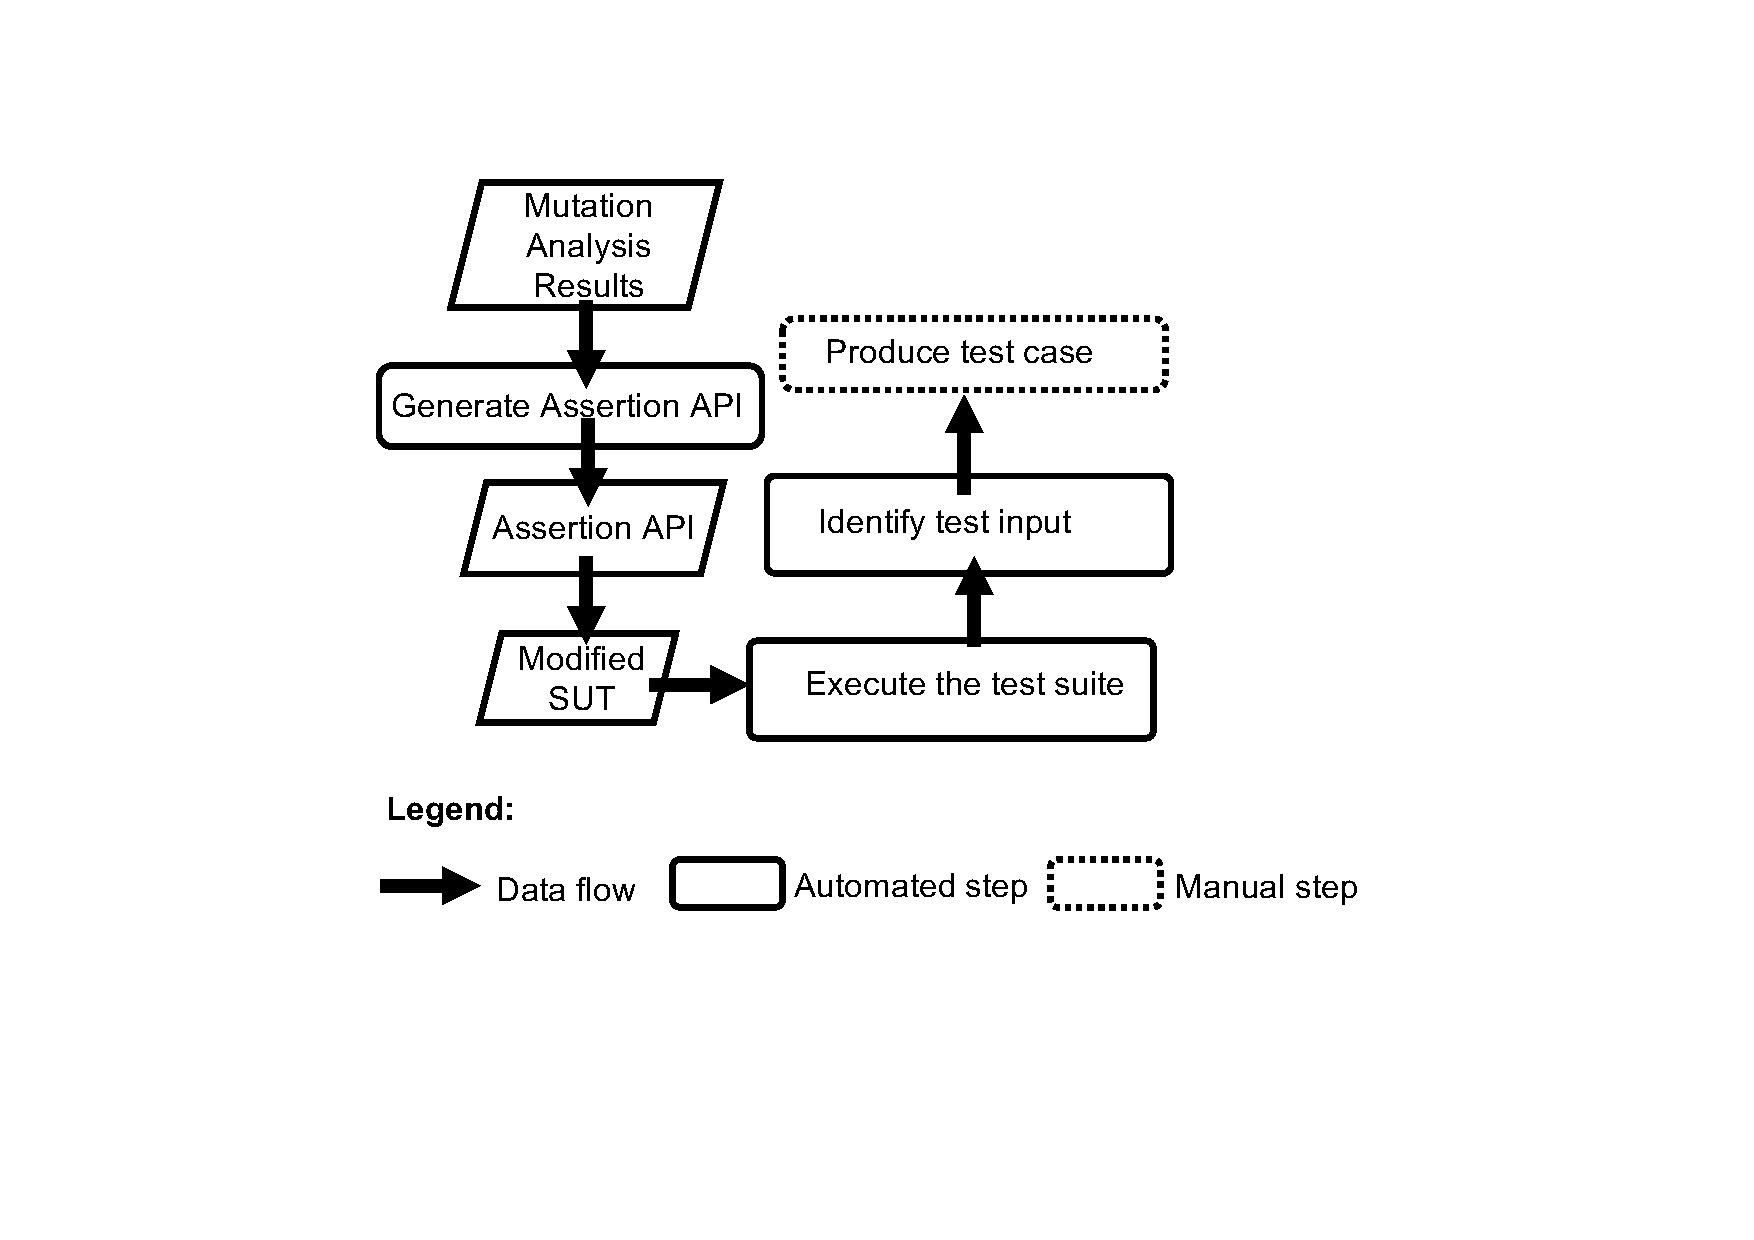
\includegraphics[width=12cm]{images/dataDrivenAugProcess}
			\caption{Data-driven Mutation Testing Process: Augmentation}
			\label{fig:data:process_aug}
		\end{figure}

\clearpage

\section{General Constraints}

\REVISION{P-3}{\RQ{} Test suite evaluation for code-driven mutation testing shall be based on SRCIror\footnote{https://github.com/TestingResearchIllinois/srciror} (detailed motivation is provided in D2).}

\RQ{} The automated generation of test cases (i.e., the objective of test suite augmentation) shall rely on existing tools because it is an open, complex, research problem.

\RQ{} The automated generation of test cases for code-mutation may rely on KLEE, which is the most stable test case generation tool, based on WP2 evaluation.


\section{Software Architecture}

\RQ{} \REVISION{P-4}{\FAQAS shall follow a modular architecture. The FAQAS Architecture is depicted in Figure~\ref{fig:architecture}. The FAQAS system shall consists of four components
\begin{itemize}
\item MASS (Mutation Analysis for Space Software), which implements test suite evaluation based on code-driven mutation.
\item SEMuS (Symbolic Execution-based Mutation testing for Space), which implements test suite augmentation based on code-driven mutation.
\item DAMAt (Data-driven Mutation Analysis), which implements test suite evaluation based on data-driven mutation.
\item DAMTE (DAta-driven Mutation TEsting), which implements test suite augmentation based on data-driven mutation.
\end{itemize}}

\RQ{} \REVISION{P-4}{At high-level, the four \FAQAS components shall work as follows. All the components receive as input the software under test (SUT), the test suite to evaluate (SUT Test Suite), and a set of configurations. MASS generates a set of code-driven mutants, the mutation score, and a list of live mutants. SEMuS receive as input the list of live mutants and generate test cases that kill them. DAMAt generates a set of data-driven mutants, the mutation score, and a list of live mutants. DAMTE receive as input the list of live data-driven mutants and generate test cases that kill them.}

\begin{figure}[h]
	\centering
		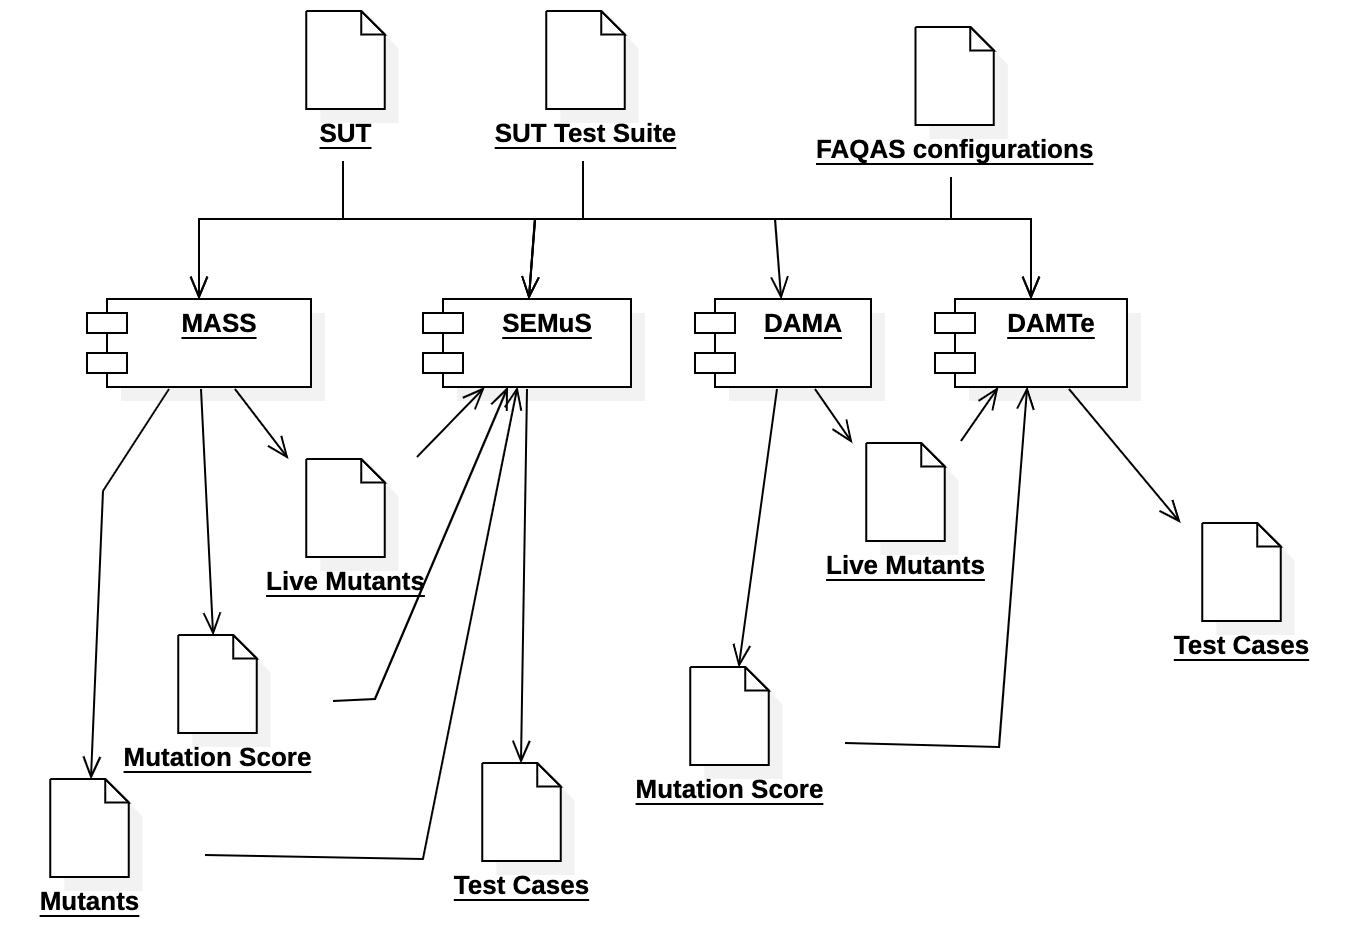
\includegraphics[width=12cm]{images/Architecture}
		\caption{FAQAS Architecture. Arrows represent data-flow.}
		\label{fig:architecture}
	\end{figure}

\clearpage
\section{Operational Environment}

\RQ{} \REVISION{P-5}{The \FAQAS shall run on any operating system provided that a bash shell and Python 3 are installed on it.}

\RQ{} The \FAQAS shall provide support to work on HPC infrastructure.

\RQ{} The \FAQAS shall be executed on the following minimum hardware specifications: 4 GB RAM and 10 GB of free disk space.

%\RQ{} The \FAQAS shall be executed on a Linux operating system with a Bash shell.

\RQ{} The \FAQAS shall be tested to work on the following Linux distributions: (i) Debian 9, (ii) Ubuntu 16, and (iii) CentOS 7.



\section{Assumptions and dependencies}

\RQ{} The \FAQAS shall process SUT built using either GCC Make~\footnote{https://gcc.gnu.org/onlinedocs/gccint/Makefile.html} or WAF\footnote{https://waf.io/}.

\REVISION{P-7}{\RQ{} The \FAQAS shall process SUT compiled with GCC~\footnote{https://gcc.gnu.org} versions above 4. }
%4.2.1, 5.4.0, and 6.3.0.

\RQ{} The \FAQAS shall process SUT test suites implemented as scripts (hereafter, \emph{test suite script}) that trigger the execution of test cases (each test case is executed in a separate process). Test suite scripts could be implemented either as Makefiles or a Bash scripts. Each test case is executed through the invocation of a command in the script.



\chapter{Requirements}

\section{Functional requirements}
\label{sec:requirements}

% !TEX root = MAIN.tex


\subsection{Test Suite Evaluation Based on Code-driven Mutation}
\label{sec:codeDriven}

The following requirements regard the Test Suite Evaluation Based on Code-Mutation functionality of the \FAQAS.



\RQ{} The \FAQAS shall implement a set of optimizations to make code-driven mutation testing feasible (see D2).

\RQ{} The \FAQAS shall implement the following optimization steps:
\begin{enumerate}
	\item Generate mutants based on code coverage;
	\item Generate mutants based on the sufficient set of operators;
	\item Discard equivalent and redundant mutants based on trivial compiler optimizations;
	\item Sample mutants based on proportional uniform sampling, proportional method-based sampling, uniform fixed-size sampling, and uniform FSCI sampling;
	\item Execute test suites prioritized and reduced based on code coverage;
	\item Discard equivalent mutants based on code coverage.
\end{enumerate}

\RQ{} The \FAQAS shall provide means to enable engineers to run code-driven mutation testing on the SUT.

\RQ{} The \FAQAS shall provide means to enable engineers to select the optimization steps to be carried on the SUT.
%\DONE{I think first we should indicate what are the optimizations supported by FAQAS}

\RQ{} The \FAQAS shall receive as input code coverage information of the SUT.

\RQ{} The \FAQAS shall support test case execution following the practice for the SUT (e.g., running the command \texttt{make test}).

\RQ{} The \FAQAS shall mutate the source code of the SUT.

\RQ{} The \FAQAS shall support C-coded software.

\RQ{} The \FAQAS shall mutate the SUT by applying a set of mutation operators that can be selected by the engineer.

\RQ{} The \FAQAS shall implement the set of operators listed in Table~\ref{table:operators}.

% !TEX root =  ../Main.tex

\newcommand{\op}{\mathit{op}}
\newcommand{\ArithmeticSet}{ \texttt{+}, \texttt{-}, \texttt{*}, \texttt{/}, \texttt{\%} }
\newcommand{\LogicalSet}{ \texttt{&&}, \texttt{||} }
\newcommand{\RelationalSet}{ \texttt{>}, \texttt{>=}, \texttt{<}, \texttt{<=}, \texttt{==}, \texttt{!=} }
\newcommand{\BitWiseSet}{ \texttt{\&}, \texttt{|}, \land }
\newcommand{\ShiftSet}{ \texttt{>>}, \texttt{<<} }


\begin{table}[h]
\caption{Implemented set of mutation operators.}
\label{table:operators} 
\centering
\scriptsize
\begin{tabular}{|@{}p{4mm}@{}|@{}p{2cm}@{\hspace{1pt}}|@{}p{11.1cm}@{}|}
\hline
&\textbf{Operator} & \textbf{Description$^{*}$} \\
\hline
\multirow{7}{*}{\rotatebox{90}{\emph{Sufficient Set}}}&ABS               & $\{(v, -v)\}$	\\
\cline{2-3}
&AOR               & $\{(\op_1, op_2) \,|\, \op_1, \op_2 \in \{ \ArithmeticSet \} \land \op_1 \neq \op_2 \} $       \\
&    			  & $\{(\op_1, \op_2) \,|\, \op_1, \op_2 \in \{\texttt{+=}, \texttt{-=}, \texttt{*=}, \texttt{/=}, \texttt{\%} \texttt{=}\} \land \op_1 \neq \op_2 \} $       \\
\cline{2-3}
&ICR               & $\{i, x) \,|\, x \in \{1, -1, 0, i + 1, i - 1, -i\}\}$           \\
\cline{2-3}
&LCR               & $\{(\op_1, \op_2) \,|\, \op_1, \op_2 \in \{ \texttt{\&\&}, || \} \land \op_1 \neq \op_2 \}$            \\
&				  & $\{(\op_1, \op_2) \,|\, \op_1, \op_2 \in \{ \texttt{\&=}, \texttt{|=}, \texttt{\&=}\} \land \op_1 \neq \op_2 \}$            \\
&				  & $\{(\op_1, \op_2) \,|\, \op_1, \op_2 \in \{ \texttt{\&}, \texttt{|}, \texttt{\&\&}\} \land \op_1 \neq \op_2 \}$            \\
\cline{2-3}
&ROR               & $\{(\op_1, \op_2) \,|\, \op_1, \op_2 \in \{ \RelationalSet \}\}$            \\
&				  & $\{ (e, !(e)) \,|\, e \in \{\texttt{if(e)}, \texttt{while(e)}\} \}$ \\
\cline{2-3}
&SDL               & $\{(s, \texttt{remove}(s))\}$            \\
\cline{2-3}
&UOI               & $\{ (v, \texttt{--}v), (v, v\texttt{--}), (v, \texttt{++}v), (v, v\texttt{++}) \}$            \\   
\hline
\hline
\multirow{5}{*}{\rotatebox{90}{\emph{OODL}}}&AOD               & $\{((t_1\,op\,t_2), t_1), ((t_1\,op\,t_2), t_2) \,|\, op \in \{ \ArithmeticSet \} $       \\ 
\cline{2-3}
&LOD               & $\{((t_1\,op\,t_2), t_1), ((t_1\,op\,t_2), t_2) \,|\, op \in \{  \} \}$       \\ 
\cline{2-3}
&ROD               & $\{((t_1\,op\,t_2), t_1), ((t_1\,op\,t_2), t_2) \,|\, op \in \{ \RelationalSet \} \}$       \\ 
\cline{2-3}
&BOD               & $\{((t_1\,op\,t_2), t_1), ((t_1\,op\,t_2), t_2) \,|\, op \in \{ \BitWiseSet \} \}$       \\ 
\cline{2-3}
&SOD               & $\{((t_1\,op\,t_2), t_1), ((t_1\,op\,t_2), t_2) \,|\, op \in \{ \ShiftSet \} \}$       \\ 
%\hline
%COR               & $\{(\op_1, \op_2) \,|\, \op_1, \op_2 \in \{ \texttt{\&\&}, \texttt{||}, \land \} \land \op_1 \neq \op_2 \}$            \\
\hline
\hline
\multirow{3}{*}{\rotatebox{90}{\emph{Other}}}&LVR			& $\{(l_1, l_2) \,|\, (l_1, l_2) \in \{(0,-1), (l_1,-l_1), (l_1, 0), (\mathit{true}, \mathit{false}), (\mathit{false}, \mathit{true})\}\}$\\
&&\\
&&\\
\hline
\end{tabular}

$^{*}$Each pair in parenthesis shows how a program element is modified by the mutation operator. Th eleft element of the pair is replaced with the right element. We follow standard syntax~\cite{kintis2018effective}. Program elements are literals ($l$), integer literals ($i$), boolean expressions ($e$), operators ($\op$), statements ($s$), variables ($v$), and terms ( $t_i$, which might be either variables or literals).
\end{table}

\RQ{} The \FAQAS shall apply all available mutation operators in case they are not specified. 

\RQN{-a} The \FAQAS shall generate all the mutants defined by each operator to be applied. 

\RQ{} The \FAQAS shall store every generated mutant on a directory tree that follows the structure of the source directory tree of the SUT.

\remark Every source file is replaced by a folder; the folder has the same name of the file. The folder contains all the mutants generated for that file.

\RQ{} The \FAQAS shall generate mutants with unique name identifiers.

\RQ{} The \FAQAS shall generate mutants with names that results from the conjunction of the following information:
source file name, mutated function name, mutated line, mutation operator name, mutation operation, mutated ``column'' (i.e., char position from the beginning of the line).

\RQ{} The \FAQAS shall compile mutants incrementally to save compilation time.

\RQ{} The \FAQAS shall disregard equivalent and redundant mutants based on trivial compiler equivalence.

% not sure if we should keep this
\RQ{} The \FAQAS shall work with compilation scripts that are modified by the engineer according to rules specific for the \FAQAS.
%Fabrizio: the subject should always be FAQAS
%The engineer shall provide a modified compilation script for the SUT (e.g., the \emph{Makefile}).
The modified compilation script (i) shall not contain debugging nor coverage flags, (ii) shall contain a placeholder for the compiler optimization option, and (iii) shall contain a 'sort' command in the source dependency list to ensure that source files are always compiled in the same order.

\RQ{} The \FAQAS shall compile every mutant with the \textit{O0}, \textit{O1}, \textit{O2}, \textit{O3}, \textit{Ofast}, and \textit{Os} GCC compiler optimisation options\footnote{https://gcc.gnu.org/onlinedocs/gcc/Optimize-Options.html}.

\RQ{} The \FAQAS shall generate a SHA512 hash for every compiled mutant to enable mutant comparisons.

\RQ{} The \FAQAS shall disregard mutants that generate a compilation error.

\RQ{} The \FAQAS shall not disregard mutants that produce a compilation warning.

\RQ{} The \FAQAS shall a produce a list of nonequivalent and nonredundant mutants based on trivial compiler equivalence.

%Fabrizio: it was fitting the implementation, not the problem to address
\RQ{} The \FAQAS shall generate a set of prioritized and reduced test suites for every mutant.
%covered statement within the SUT.
The generation of such test suites should be  based on the PrioritizeAndReduce Algorithm (See D2).

\RQ{} The \FAQAS shall provide an option to execute only the prioritized and reduced set of test cases when testing a mutant affecting a certain statement. When the option is disabled, the \FAQAS shall execute the whole test suite for every mutant. The execution of a test suite shall be stopped when a mutant is killed.

\RQ{} The \FAQAS shall support strong mutation testing (see D2).

\RQ{} The \FAQAS shall sample the mutants to be executed.

\RQ{} The \FAQAS shall support the mutant selection strategy \textit{all mutants} (see D2).

\RQ{} The \FAQAS shall support the mutant selection strategy \textit{proportional uniform sampling} (see D2).

\RQ{} The \FAQAS shall support the mutant selection strategy \textit{proportional method-based sampling} (see D2).

\RQ{} The \FAQAS shall enable engineers to provide a sampling rate if \textit{proportional uniform sampling} or \textit{proportional method-based sampling} is selected.

\RQ{} The \FAQAS shall support the mutant selection strategy \textit{uniform FSCI sampling} (see D2).

\RQ{} The \FAQAS shall compile a mutant by running the build script of the original program.

\RQ{} The \FAQAS shall support simple runtime optimizations:
\begin{enumerate}
	\item stopping the execution of the test suite when the mutant has been killed,
	\item executing only those test cases that cover the mutated statements, and
	\item rely on timeouts to automatically detect infinite loops introduced by mutation.
\end{enumerate}

%\RQ{} The \FAQAS shall execute the SUT test suite for every mutant.

\RQ{} The \FAQAS shall compile and execute mutants till a termination criterion is met. The termination criterion depends on the mutants selection strategy (see D2 for details):
\begin{itemize}
	\item \emph{all mutants}: all mutants have been executed
	\item \emph{proportional uniform sampling}: a number of mutants matching the selected percentage has been executed
	\item \emph{proportional method-based sampling}: a number of mutants matching the selected percentage for all methods in the SUT has been executed
	\item \emph{uniform fixed-size sampling}: a number of mutants matching the selected value has been executed
	\item \emph{uniform FSCI sampling}: the confidence interval computed is smaller than 10\%.
\end{itemize}


\RQ{} The \FAQAS shall identify equivalent mutants based on code coverage information using the distance criterion $D_C$ (see D2).

%\RQ{} The \FAQAS shall disregard all the equivalent mutants from the mutation results.

\RQ{} The \FAQAS shall compute the mutation score of the SUT based on mutation results. Equivalent mutants shall not be considered for the computation of the mutation score (see D2).

\RQ{} The \FAQAS shall produce two prioritized lists (list A and list B) of live and nonequivalent mutants.
%\TODO{We have to discuss the meaning of the following sentence}
List A shall contain live mutants that are different from the SUT (i.e., nonequivalent) and different from each other. Ideally, each mutant in list A should represent a distinct limitation of the SUT.
List A contains mutants that have a distance $D_C$ (strictly) greater than zero; in other words, the distance between each pair of mutants appearing in list A should be greater than zero.
List B contains all the remaining live, nonequivalent mutants.
The two lists are sorted in decreasing order, based on the distance $D_C$ from the original program.

\remark Equivalent mutants, which are discarded, have a distance $D_C$ from the original program equal to zero.
The generation of the list proceeds as follows. First, a list (list X) containing all the mutants, sorted by distance $D_C$, is created. Iteratively, each mutant in list X is compared with each mutant in list A. If the distance is greater than zero, the mutant is added to list A, otherwise it is added to list B.


\RQ{} The \FAQAS shall report a summary of the results obtained in every step of the mutation testing process. \REVISION{P-12}{The generated reports shall include information about the total number of mutants generated, the total number of mutants filtered by compiler optimisations, the type of mutants sampling employed, the total number of mutants executed, the total number of killed mutants, the total number of live mutants, the mutation score, the statement coverage, and the location of the two prioritized lists of nonequivalent mutants.}


% test suite augmentation


\subsection{Test Suite Augmentation Based on Code-driven Mutation}
\label{sec:codeDrivenAugmentation}

The following requirements regard the Test Suite Augmentation functionality aiming to generate test cases that kill mutants generated with the Code-driven Mutation functionality of the \FAQAS.

\RQ{} The \FAQAS shall support test suite augmentation based on code mutation.

\RQ{} The \FAQAS shall rely on the KLEE test case generation tool to support test suite augmentation.

\RQ{} For each live mutant, the \FAQAS should generate test scaffoldings that are processed by KLEE.

\RQ{} The \FAQAS shall provide the engineer with the ability to configure the generated test scaffoldings.


\remark For example, the \FAQAS shall provide the engineer with the ability to refine the generated assertions. Since assertions concern output and state variables, it is necessary to verify that all the necessary output/state variables had been referred in assertion. Indeed, in C, with pointers and pointers to pointers, it is not possible to have a precise automated identification of output/state variables.

\RQ{} The \FAQAS shall generate a tentative unit test case (i.e., a source file in C) that kills the mutants.

\remark  The \FAQAS may generate test cases consisting of (i) an invocation of the function under test (i.e., the function targeted by the mutation), (ii) its assigned arguments, and (iii) an assertion that verifies results.

%\RQ{} The engineer shall inspect the generated test cases by verifying that KLEE has generated valid inputs (e.g., inputs that meet the program preconditions).
%
%\RQ{} The engineer shall inspect the generated test cases by verifying that the generated assertion with the expected value is correct (i.e., it reflects what indicated in the SUT specifications).
%
%\remark If the value appearing in the assertion is not correct, it means that KLEE during its execution has observed an incorrect value being generated by the SUT; for this reason, the SUT might be faulty and should be fixed.
%
%\RQ{} The engineer shall add manually the generated test case to the test suite.
%
%\RQ{} The engineer shall inspect manually the mutant for equivalence when a test case is not generated.
%
%\RQ{} The engineer shall remove the mutant from the mutation results, if the manual inspection of mutant equivalence is positive.
%
%\RQ{} The \FAQAS shall recompute the mutation score after ignoring the equivalent mutants detected by KLEE.

% !TEX root = MAIN.tex


\subsection{Test Suite Evaluation Based on Data-driven Mutation}
\label{sec:dataDriven}

The following requirements regard the Test Suite Evaluation Based on the Data-driven Mutation Testing functionality of the \FAQAS.



\RQ{} The \FAQAS shall work with a fault model and a data model for the SUT specified according to D2.

\RQ{} The \FAQAS shall provide a mutation analysis API (i.e., predefined functions to perform data mutation for buffers).

\RQ{} The \FAQAS shall automatically generate the data mutation probes to be integrated within the SUT.

\RQ{} The engineer shall manually modify the source code of the SUT to integrate mutation probes into it.

\REVTOOL{P-11}{\RQ{} The \FAQAS shall support C-coded software and C++-coded software.}

%\RQ{} The \FAQAS shall require the engineer to manually modify the scripts used to execute test cases so they include an invocation to \FAQAS after the execution of every single test case.
%
%\RQ{} The \FAQAS shall receive as inputs the command to compile the SUT, the command to execute the test suite, the path to the extended SUT source code, and the mutants selection configuration.

\RQ{} The \FAQAS shall provide the engineer with the ability to choose to mutate all the instances of the data item, one instance of the data item, or a percentage of the instances.

% \RQ{} The \FAQAS shall mutate the target data item by applying a set of mutation operations derived by a set of mutation operators that shall be specified by the engineer in the Fault Model.

\REVTOOL{P-11}{\RQ{} The \FAQAS shall implement the set of operators listed in Table~\ref{table:damat:operators}.}

% !TEX root = ../MAIN.tex

\newcommand{\MINIPM}{3cm}
\newcommand{\MINIPW}{10cm}

\begin{table*}[h]
\caption{Data-driven mutation operators}
\label{table:operators}
\scriptsize
\begin{tabular}{|p{15mm}|p{10mm}|p{3cm}|p{10cm}|}
\hline
\textbf{Fault Class}&\textbf{Types}&\textbf{Parameters}&\textbf{Description}\\
\hline
Value above threshold (VAT)&
I,L,F,D,H
&
\begin{minipage}{\MINIPM}
T: threshold\\
\D: delta, difference with respect to threshold\\
\end{minipage}
&
\begin{minipage}{\MINIPW}
Replaces the current value with a value above the threshold T for a delta (\D). It simulates a value that is out of the nominal case and shall trigger a response from the system that shall be verified by the test case (e.g., the system may continue working but an alarm shall be triggered). Not applied if the value is already above the threshold.

\EMPH{Data mutation procedure:}
$v' =  (T+\Delta)   (\mathit{if} v \le T); v' =  v   (\mathit{otherwise})$;

%\EMPH{Data mutation procedure:}
%\[
%v' =
%    \begin{cases}
%      (T+D)    & \mathit{if} v \le T\\
%      v    & \mathit{otherwise}\\
%    \end{cases}
%\]

\end{minipage}
\\



\hline
Value below threshold (VBT)&
I,L,F,D,H
&
\begin{minipage}{\MINIPM}
T: threshold\\
\D: delta, difference with respect to threshold\\
\end{minipage}
&
\begin{minipage}{\MINIPW}
Replaces the current value with a value below the threshold T for a delta (\D). It simulates a value that is out of the nominal case and shall trigger a response from the system that shall be verified by the test case (e.g., the system may continue working but an alarm shall be triggered). Not applied if the value is already below the threshold.

\EMPH{Data mutation procedure:}
$v' =  (T-\Delta)  (\mathit{if} v \ge T); v' = v    (\mathit{otherwise})$

%\EMPH{Data mutation procedure:}
%\[
%v' =
%    \begin{cases}
%      (T-D)    & \mathit{if} v \ge T\\
%      v    & \mathit{otherwise}\\
%    \end{cases}
%\]
\end{minipage}
\\



\hline
Value out of range (VOR)&
I,L,F,D,H
&
\begin{minipage}{\MINIPM}
MIN: minimum valid value\\
MAX: maximum valid value\\
\D: delta, difference with respect to minimum/maximum valid value
\end{minipage}
&
\begin{minipage}{\MINIPW}
Replaces the current value with a value out of the range $[MIN;MAX]$. It simulates a value that is out of the nominal range and shall trigger a response from the system that shall be verified by the test case (e.g., the system may continue working but an alarm shall be triggered). Not applied if the value is already out of range.

\EMPH{Data mutation procedure 1:}
$v' =  (MIN-\Delta)    (\mathit{if} MIN \le v \le MAX); v' = v   (\mathit{otherwise})$\\

\EMPH{Data mutation procedure 2:}
$v' = (MAX+\Delta)   (\mathit{if} MIN \le v \le MAX); v' = v   (\mathit{otherwise})$\\

%\EMPH{Data mutation procedure 1:}
%\[
%v' =
%    \begin{cases}
%      (MIN-D)    & \mathit{if} MIN \le v \le MAX\\
%      v    & \mathit{otherwise}\\
%    \end{cases}
%\]
%
%\EMPH{Data mutation procedure 2:}
%\[
%v' =
%    \begin{cases}
%      (MAX+D)    & \mathit{if} MIN \le v \le MAX\\
%      v    & \mathit{otherwise}\\
%    \end{cases}
%\]

\end{minipage}
\\






\hline
Bit flip (BF)&
B
&
\begin{minipage}{\MINIPM}
MIN: lower bit\\
MAX: higher bit\\
STATE: mutate only if the bit is in the given state (i.e., 0 or 1). \\
VALUE: number of bits to mutate\\
\end{minipage}
&
\begin{minipage}{\MINIPW}
A number of bits randomly chosen in the positions between MIN and MAX (included) are flipped.
If STATE is specified, the mutation is applied only if  the bit is in the specified state; the value $-1$ indicates that any state shall be considered for mutation. Parameter VALUE specifies the number of bits to mutate.

\EMPH{Data mutation procedure:} the operator flips VALUE randomly selected bit if they are in the specified state.

\end{minipage}
\\

\hline
Invalid numeric value (INV)&
I,L,F,D,H
&
\begin{minipage}{\MINIPM}
MIN: lower valid value\\
MAX: higher valid value\\
\end{minipage}
&
\begin{minipage}{\MINIPW}
Replace the current value with a mutated value that is legal (i.e., in the specified range) but different than current value. It simulates the exchange of data that is not consistent with the state of the system.

\EMPH{Data mutation procedure:} Replace the current value with a different value randomly sampled in the specified range.
\end{minipage}
\\

\hline
Illegal Value (IV)
&
I,L,F,D,H
&
\begin{minipage}{\MINIPM}
VALUE: illegal value that is observed\\
\end{minipage}
&
\begin{minipage}{\MINIPW}
Replace the current value with a value that is equal to the parameter \emph{VALUE}.

\EMPH{Data mutation procedure:}
$v' = \mathit{VALUE}    (\mathit{if} v \ne \mathit{VALUE}); v' = v   (\mathit{otherwise})$\\

%\EMPH{Data mutation procedure:}
%\[
%v' =
%    \begin{cases}
%      \mathit{VALUE}    & \mathit{if} v \ne \mathit{VALUE}\\
%      v    & \mathit{otherwise}\\
%    \end{cases}
%\]
\end{minipage}
\\

\hline
Anomalous Signal Amplitude (ASA)
&
I,L,F,D,H
&
\begin{minipage}{\MINIPM}
T: change point\\
\D: delta, value to add/remove\\
VALUE: value to multiply\\
\end{minipage}
&
\begin{minipage}{\MINIPW}
The mutated value is derived by amplifying the observed value by a factor \emph{V} and by adding/removing a constant value \D from it. It is used to either amplify or reduce a signal in a constant manner to simulate unusual signals. The parameter \emph{T} indicates the observed value below which instead of adding  we subtract .

\EMPH{Data mutation procedure:}
$v' =  T+(  (v-T)*\mathit{VALUE}  ) + \Delta  (\mathit{if}\ v \ge T); v' = T - (  (T-v)*\mathit{VALUE}  ) - \Delta   (\mathit{if}\ v < T)$;
\end{minipage}

%\EMPH{Data mutation procedure:}
%\[
%v' =
%    \begin{cases}
%      T+(  (v-T)*\mathit{VALUE}  ) + \mathit{D}    & \mathit{if}\ v \ge T\\
%      T - (  (T-v)*\mathit{VALUE}  ) - \mathit{D}   & \mathit{if}\ v < T
%    \end{cases}
%\]
%\end{minipage}
\\


\hline
Signal Shift (SS)
&
I,L,F,D,H
&
\begin{minipage}{\MINIPM}
\D: delta, value by which the signal should be shifted\\
\end{minipage}
&
\begin{minipage}{\MINIPW}
The mutated value is derived by adding a value \D to the observed value. It simulates an anomalous shift in the signal.

\EMPH{Data mutation procedure:}
$v' = v + \Delta$
\end{minipage}
\\





\hline
Hold Value (HV)
&
\begin{minipage}{\MINIPW}
I,L,F,D,H
\end{minipage}
&
\begin{minipage}{\MINIPM}
V: number of times to repeat the same value\\
\end{minipage}
&
\begin{minipage}{\MINIPW}
This operator keeps repeating an observed value for $V$ times. It emulates a constant signal replacing a signal supposed to vary.

\EMPH{Data mutation procedure:}
$v' = \mathit{previous}\  v'   (\mathit{if}\ \mathit{counter} \le V) ; v' = v  \mathit{otherwise}$

%\EMPH{Data mutation procedure:}
%\[
%v' =
%    \begin{cases}
%      \mathit{previous}\  v'   & \mathit{if}\ \mathit{counter} \le V\\
%      v  & \mathit{otherwise}\
%    \end{cases}
%\]
\end{minipage}
\\

\hline
Fix value above threshold (FVAT)&
I,L,F,D,H
&
\begin{minipage}{\MINIPM}
T: threshold\\
\D: delta, difference with respect to threshold\\
\end{minipage}
&
\begin{minipage}{\MINIPW}
It is the complement of VAT and implements the same mutation procedure as VBT but we named it differently because it has a different purpose. Indeed, it is used to verify that test cases exercising exceptional cases are verified correctly. In the presence of a value above the threshold, it replaces the current value with a value below the threshold T for a delta \D.

\EMPH{Data mutation procedure:}
$v' =  v    (\mathit{if} v > T) ; V' = (T-\Delta)    (\mathit{otherwise})$

%\EMPH{Data mutation procedure:}
%\[
%v' =
%    \begin{cases}
%      v    & \mathit{if} v > T\\
%      (T-D)    & \mathit{otherwise}\\
%    \end{cases}
%\]

\end{minipage}
\\

\hline
Fix value below threshold (FVBT)&
I,L,F,D,H
&
\begin{minipage}{\MINIPM}
T: threshold\\
\D: delta, difference with respect to threshold\\
\end{minipage}
&
\begin{minipage}{\MINIPW}
It is the counterpart of FVAT for the operator VBT.
% and implements the same mutation operation as VAT but we named it differently because it has a different purpose. Indeed, it is used to verify that test cases exercising exceptional cases are verified correctly. In the presence of a value below the threshold it replaces the current value with a value above the threshold T for a delta D.

\EMPH{Data mutation procedure:}
$v' = v   (\mathit{if} v < T); v' = (T+\Delta) (\mathit{otherwise})$\\

%\EMPH{Data mutation procedure:}
%\[
%v' =
%    \begin{cases}
%      v    & \mathit{if} v < T\\
%      (T+D)    & \mathit{otherwise}\\
%    \end{cases}
%\]

\end{minipage}
\\



\hline
Fix value out of range (FVOR)&
I,L,F,D,H
&
\begin{minipage}{\MINIPM}
MIN: minimum valid value\\
MAX: maximum valid value\\
\end{minipage}
&
\begin{minipage}{\MINIPW}
It is the complement of VOR and implements the same mutation procedure as INV but we named it differently because it has a different purpose. Indeed, it is used to verify that test cases exercising exceptional cases are verified correctly.
%In the presence of a value out of the range  $[MIN;MAX]$ it replaces the current value with a random value within the range.

\EMPH{Data mutation procedure:}
$v' = v   (\mathit{if} MIN \le v \le MAX); v' = \mathit{random(MIN,MAX)}   (\mathit{otherwise})$

%\EMPH{Data mutation procedure:}
%\[
%v' =
%    \begin{cases}
%      v    & \mathit{if} MIN \le v \le MAX\\\\
%      \mathit{random(MIN,MAX)}    & \mathit{otherwise}\\
%    \end{cases}
%\]

\end{minipage}
\\

%\hline
%\TRFOUR{Array Swap (AS)}
%&
%\begin{minipage}{\MINIPW}
%ARRAY\_*\\
%\end{minipage}
%&
%\begin{minipage}{\MINIPW}
%MIN: position of element A\\
%MAX: position of element B\\
%VALUE: number of elements to move\\
%\end{minipage}
%&
%\begin{minipage}{\MINIPW}
%Replace a number of elements (number specified by VALUE) located starting from position MIN, with a number of elements located starting from position MAX, and viceversa.
%\EMPH{Data mutation procedure:} Mutation is performed by replacing the two set of elements with each other.
%\end{minipage}
%\\
%
%
%\hline
%\TRFOUR{Array Random Swap (ARS)}
%&
%\begin{minipage}{\MINIPW}
%ARRAY\_*\\
%\end{minipage}
%&
%\begin{minipage}{\MINIPW}
%MIN: min position of element A/B\\
%MAX: max position of element A/B\\
%VALUE: number of elements to move\\
%\end{minipage}
%&
%\begin{minipage}{\MINIPW}
%Replace a number of elements (number specified by VALUE) located in a position between MIN and MAX, with a number of elements located in a position between MIN and MAX. MIN and MAX specify a position with respect to the beginning and end of the array.  For example, MIN=0 indicates the first element of teh array, MIN=-2 indicates the second element of the array.
%\EMPH{Data mutation procedure:} Mutation is performed by replacing the two set of elements with each other.
%\end{minipage}
%\\



%Incorrect Identifier& Several transmission data fields have fixed values, for example fields identifying the transmitting satellite. Hardware/software errors may assign incorrect identifiers.\\
%%Incorrect Checksum& Hardware/software errors may result in an incorrect checksum for a Packet or VCDU.\\
%Incorrect Counter& Counters are used to track Packet or VCDU ordering. Hardware/software errors may assign incorrect counter values.\\
%Flipped Data Bits& Physical channel noise may flip one or more bits in the data transmission.\\
\hline
\end{tabular}
\textbf{Legend:} I: INT, L: LONG INT, F: FLOAT, D: DOUBLE, B: BIN, H: HEX


\end{table*}%


\REVTOOL{P-11}{\RQ{} For every mutation operator defined in the Fault Model, the \FAQAS shall generate one or more mutants performing a mutation operation.}

\REVTOOL{P-11}{\RQ{} The \FAQAS shall identify each mutant with a unique numerical identifier.}

\REVTOOL{P-11}{\RQ{} The \FAQAS will automatically generate a table containing the definition of all the generated mutants and their identifiers.}

\RQ{} The \FAQAS shall work with compilation scripts that are modified by the engineer according to rules specific for the \FAQAS.

\RQ{} The \FAQAS shall enable the compilation of a version of the SUT that traces the data items (targeted by mutation) that are covered by each test case.

\RQ{} The \FAQAS shall derive, from logs generated during the execution of the SUT test suite, the data items exercised by each test case.

\REVTOOL{P-11}{\RQ{} The \FAQAS shall provide, for each mutant, a list of all test cases covering the data item targeted by the mutant.
}
\RQ{} The \FAQAS shall compile a version of the SUT for every generated mutant.

\RQ{} For each mutation operator, the \FAQAS shall execute only the test cases exercising the data item targeted by the mutation operator.

\REVTOOL{P-11}{\RQ{} The \FAQAS shall execute every mutant against all the test cases exercising the data item targeted by the mutation operator.
}
\REVTOOL{P-11}{\RQ{} The \FAQAS shall support test case execution following the practice for the SUT (e.g., running the command \texttt{make test}).
}
\RQ{} For each mutation operation, the \FAQAS shall provide the engineer with information on the number of instances of the data item that have been mutated and not mutated by the selected mutation operation.

\RQ{} The \FAQAS shall automatically determine if the mutation operation has been performed at least once.

\RQ{} The \FAQAS shall automatically determine if a mutant has been killed.

\REVTOOL{P-11}{\RQ{} The \FAQAS shall compute the fault model coverage (see D2) on the mutation results.
}
\REVTOOL{P-11}{\RQ{} The \FAQAS shall compute the mutation operation coverage (see D2) on the mutation results.
}
\RQ{} The \FAQAS shall compute the mutation score (see D2) based on the mutation results.

\REVTOOL{P-11}{\RQ{} The \FAQAS shall produce a list of all the mutants and their status.
}
\REVTOOL{P-11}{\RQ{} The \FAQAS shall describe the status of a mutant relative to the Fault Model Coverage as \texttt{COVERED}, if the or \texttt{NOT\_COVERED}.
}
\REVTOOL{P-11}{\RQ{} The \FAQAS shall mark all mutants targeting a data item exercised by the test suite as \texttt{COVERED}.
}
\REVTOOL{P-11}{\RQ{} The \FAQAS shall mark all mutants targeting a data item not exercised by the test suite as \texttt{NOT\_COVERED}
}
\REVTOOL{P-11}{\RQ{} The \FAQAS shall describe the status of a mutant relative to the Mutation Operation Coverage as \texttt{APPLIED} or \texttt{NOT\_APPLIED}.
}
\REVTOOL{P-11}{\RQ{} The \FAQAS shall mark all mutants that performed the corresponding mutation operation at least once as \texttt{APPLIED}
}
\REVTOOL{P-11}{\RQ{} The \FAQAS shall mark all mutants that did not perform the corresponding mutation operation at least once as \texttt{NOT\_APPLIED}.
}
\REVTOOL{P-11}{\RQ{} The \FAQAS shall describe the status of a mutant relative to the Mutation Score as \texttt{KILLED} or \texttt{LIVE}.
}
\REVTOOL{P-11}{\RQ{} The \FAQAS shall mark all mutants that caused at least a test case failure as \texttt{KILLED}.
}
\REVTOOL{P-11}{\RQ{} The \FAQAS shall mark all mutants that did not cause at least a test case failure as \texttt{LIVE}.
}
\RQ{} The \FAQAS shall provide the engineer with the means to inspect the mutation results. The \FAQAS data-driven mutation results shall include the list of data types not covered by any test case, the list of data types exercised by each test case, the list of live and killed mutants, and the result of every executed test case.

%\RQ{} The data-driven mutation testing component from \FAQAS shall not implement any feature to automatically generate test cases.

\subsection{Test Suite Augmentation Based on Data-driven Mutation}
\label{sec:codeDrivenAugmentation}

The following requirements regard the Test Suite Augmentation functionality that aims to generate test cases that kill mutants generated with the Data-driven Mutation functionality of the \FAQAS.

\RQ{} The \FAQAS shall generate a version of the testing API that shall contain reachability assertions that enable KLEE to generate inputs that reach the mutation.

\RQ{} The \FAQAS shall not fully automate the Data-driven Test Suite Augmentation functionality.

\remark The engineer shall execute KLEE, after performing the required scaffolding, if necessary.
Also, the engineer shall implement a test case based on KLEE's output.




\section{System interface requirements}

\RQ{} The user interface of the \FAQAS is provided through the command line.

\REVISION{P-15a}{\RQ{} The \FAQAS shall process code coverage information recorded using the format of \texttt{gcov}\footnote{https://gcc.gnu.org/onlinedocs/gcc/Gcov.html}.

\REVISION{P-15a}{\RQ{} The \FAQAS shall automatically execute gcov, when available, to generate code coverage information.}


\REVISION{P-15c}{\RQ{} The \FAQAS shall support the following commands:
\begin{itemize}
	\item \texttt{MASS}:
	\begin{itemize}
		\item \texttt{PrepareSUT}: command to prepare the SUT and collect information about the SUT test suite.
		\item \texttt{GenerateMutants}: command to generate mutants from the SUT source code.
		\item \texttt{CompileOptimizedMutants}: command to compile the mutants with the multiple optimisation levels.
		\item \texttt{OptimizedPostProcessing}: command to disregard equivalent and redundant mutants based on compiler optimisations.
		\item \texttt{GeneratePTS}: command to generate the prioritized and reduced test suites.
		\item \texttt{ExecuteMutants}: command to execute mutants against the SUT test suite.
		\item \texttt{IdentifyEquivalents}: command to identify equivalent mutants based on code coverage.
		\item \texttt{MutationScore}: command to compute the mutation score and final reporting.
		\item \texttt{PrepareMutants\_HPC}: command to prepare the mutants workspace for the execution on HPCs.
		\item \texttt{ExecuteMutants\_HPC}: command to execute mutants on HPCs.
		\item \texttt{PostMutation\_HPC}: command to assess past mutant executions, and to decide whether more mutant executions are needed.
	\end{itemize}
\REVTOOL{P-11}{	\item \texttt{DAMAt}:
	\begin{itemize}
		\item \texttt{DAMAt\_probe\_generation}: command to generate the data mutation probes.
		\item \texttt{DAMAt\_mutants\_launcher}: command to execute the mutants against the SUT. test suite.
	\end{itemize}}
\end{itemize}
}

\REVISION{P-15b}{\RQ{} The \FAQAS shall generate the following log files:
\begin{itemize}
	\item \texttt{MASS}
	\begin{itemize}
		\item output concerning SUT compilation process
		\item output concerning execution of SUT test cases
		\item output concerning the execution of the \texttt{CompileOptimizedMutants} command
		\item output concerning the execution of the \texttt{OptimizedPostProcessing} command
		\item output concerning the execution of the \texttt{GeneratePTS} command
		\item output concerning the execution of the \texttt{ExecuteMutants} command
		\item output concerning the execution of the \texttt{IdentifyEquivalents} command
		\item output concerning the execution of the \texttt{MutationScore} command
		\item output concerning the execution of the \texttt{PrepareMutants\_HPC} command
		\item output concerning the execution of the \texttt{ExecuteMutants\_HPC} command
		\item output concerning the execution of the \texttt{PostMutation\_HPC} command
	\end{itemize}
\REVTOOL{P-11}{	\item \texttt{DAMAt}
	\begin{itemize}
		\item output concerning the execution of the \texttt{DAMAt\_probe\_generation} command
		\item output concerning the execution of the \texttt{DAMAt\_mutants\_launcher} command
	\end{itemize}}
\end{itemize}

}

\REVISION{P-15d}{
\RQ{} The \FAQAS shall be configured through texts files.
%named \texttt{mass\_conf.sh
}

\RQ{} The \FAQAS configuration file shall be set with the following parameters:
	\begin{itemize}
		\item \FAQAS installation path
		\item \FAQAS workspace path
		\item SUT relevant paths (e.g., source code folder, test folder, coverage folder)
		\item SUT compilation command
		\item SUT test case execution command
		\item \FAQAS execution environment mode (i.e., single machine, HPC)
		\item \FAQAS trivial compiler optimisation flags
		\item \FAQAS sampling type
		\item \FAQAS sampling rate
		\item \FAQAS test suite prioritization type
	\end{itemize}
}

\RQ{} The \FAQAS shall provide built-in features to process the SUT test harness Google Test\footnote{https://github.com/google/googletest} and the Basic mathematical Library Test Suite (BLTS)\footnote{https://essr.esa.int/project/mlfs-mathematical-library-for-flight-software}.

\REVISION{P-16}{\RQ{} The \FAQAS shall provide means to configure its execution with any test harness infrastructure for C/C++ software.}

\RQ{} The \FAQAS shall provide the engineer with the ability to configure the environment variables used to tune the mutation testing process.

\section{Adaptation and missionization requirements}

\RQ{} The \FAQAS shall not be used in flight. Precisely, it shall not be executed to test software running on a spacecraft hardware on orbit.

\RQ{} The \FAQAS shall be used in the development environment.




\section{Computer resource requirements}


\RQ{} The \FAQAS shall run on Linux operating systems.



\section{Security requirements }

\RQ{} The \FAQAS shall not use network connections.

\section{Safety requirements}

\RQ{} The \FAQAS should not be used to assess test cases that are executed with target hardware in the loop, to avoid safety hazards.

\section{Reliability and availability requirements}

\RQ{} The \FAQAS shall work according to its functional specifications every time it is invoked.

% \RQ{} The system is expected to work according to is functional specifications every time it is invoked.

\RQ{} The \FAQAS shall not provide an upper bound for mutation testing execution time.

\remark Mutation testing execution time depends on both the number of mutants to be executed and the duration of the test suite execution, information that cannot be foreseen before execution.

\section{Quality requirements}

\RQ{} Usability. Software engineers shall be able to successfully use the \FAQAS after reading its documentation.

\RQ{} The \FAQAS shall be used in any environment matching the characteristics indicated in this document.

\RQ{} The \FAQAS shall comply with software development standards. The software development process shall follow ECSS guidelines as per SoW.


\section{Design requirements and constraints}

\RQ{} The \FAQAS shall be released with ESA Software Community Licence Permissive – v2.3, as defined at https://essr.esa.int/. Any reused component should be compatible with the abovementioned licence.

\RQ{} The \FAQAS shall be implemented using the bash shell script language, the Python programming language, and the C/C++ programming language.

\RQ{} \FAQAS shall mutate the source code of the SUT not the intermediate representation.


\section{Adaptation and installation requirements}

% - Deployment methods (it is maybe a bit early, but we have to think on the methodology to deploy the tool e.g. compile it, have it delivered with an installer, on a container, etc)

%
\RQ{} The \FAQAS should be installed using an installer software.


\section{Software operations requirements}

\RQ{} The \FAQAS shall be executed at anytime,
%It should be possible to execute the system anytime,
in an environment matching the characteristics indicated in this document.

\section{Software maintenance requirements}

\RQ{} One year maintenance support shall be provided as per SoW.

\section{System and software observability requirements}

\RQ{} The debugging of the \FAQAS shall be possible if and only if
%To enable post-mortem debugging,
all the temporary files generated by the system are kept.

\chapter{Verification, validation and system integration}
 \section{Verification and validation process requirements}

\RQ{} Every mutation operator implemented by the \FAQAS shall be tested by a dedicated unit test case.

% \RQ{} Unit test cases shall be executed on a x86-64 desktop PC.

% \RQ{} Unit test cases execution time shall not exceed one day.

% \RQ{} A system test suite for the Code-Driven Mutation Testing component shall be provided. The Code-Driven Mutation Testing component shall be tested as a whole based on the MLFS case study (see D2).

 \RQ{} The \FAQAS shall enable the correct computation of the mutation score for the FAQAS case study systems indicated in deliverable D2.

% \TODO{Questi che seguono li avevi dimenticati giusto?}
% \DONE{Non veramente, due c'erano gia', ma gli altri li hai scritto meglio, cmq ho fixato}

\RQ{}  \REVISION{SUTP-4}{Since in the \FAQAS units are self-contained (i.e., they do not interact with other units but simply store results in files processed by other units), the integration of pairs of unit shall not be tested.}

\RQ{} \REVISION{SUTP-4}{The \FAQAS shall be tested as a whole, based on tutorial examples described in SUM.}

\RQ{} \REVISION{SUTP-5}{Unit test cases shall be executed on a x86-64 desktop PC.}

\RQ{} \REVISION{SUTP-5}{Unit test cases execution time should not exceed one day.}

 \subsection{Validation approach}



\RQ{} SnT shall perform a preliminary validation of the delivered framework.

\RQ{} FAQAS industry partners shall use the system at their premises to validate it.
